%
% Modelo de trabalho acadêmico (Teses, Dissertações, TCC)
% Documento principal
%
% Centro Federal de Educação Tecnológica de Minas Gerais - CEFET-MG
% Autor: Cristiano Fraga G. Nunes <cfgnunes@gmail.com>
%
%
% Projeto hospedado em: https://github.com/cfgnunes/latex-cefet-mg
%

% Largura da tabulação dos arquivos igual a 8 (utilizar 'Tab' ao invés de 'Espaços')
% TODO: criar glossário
% TODO: criar índice remissivo

\documentclass{abntex2-cefetmg}

% importações de pacotes
	\usepackage[alf, abnt-emphasize=bf, bibjustif, recuo=0cm, abnt-etal-cite=2, abnt-etal-list=0]{abntex2cite}	% citações padrão ABNT
	\usepackage{bookmark}					% cria menu de bookmarks
	\usepackage[utf8]{inputenc}				% acentuação direta
	\usepackage[T1]{fontenc}				% codificação da fonte em 8 bits
	\usepackage[dvips]{graphicx}				% inserir figuras
	\usepackage{amsfonts, amssymb, amsmath, dsfont}		% fonte e simbolos matemáticos
	\usepackage{booktabs}					% comandos para tabelas
	\usepackage{verbatim}					% texto é interpretado como escrito no documento
	\usepackage{multirow, array}				% múltiplas linhas e colunas em tabelas
	\usepackage[bottom]{footmisc}				% mantem as notas de rodapé sempre na mesma posicao
	\usepackage{indentfirst}				% indenta o primeiro parágrafo de cada seção.
	\usepackage{microtype}					% para melhorias de justificação?
	\usepackage{palatino}					% usa a fonte Palatino
	%\usepackage{times}					% usa a fonte Times
	%\usepackage{lmodern}					% usa a fonte Latin Modern
	%\usepackage{subfig}					% posicionamento de figuras
	%\usepackage[algoruled, portuguese]{algorithm2e}	% escrever algoritmos
	%\usepackage{acronym}					% produzir acrônimos
	%\usepackage{scalefnt}					% permite redimensionar tamanho da fonte
	%\usepackage{color, colortbl}				% comandos de cores
	%\usepackage{lscape}					% permite páginas em modo "paisagem"
	%\usepackage{breakurl}					% permite quebra de linha em urls
	%\usepackage{ae,aecompl}				% fontes de alta qualidade
	%\usepackage{picinpar}					% dispor imagens em parágrafos
	%\usepackage{latexsym}					% simbolos matematicos
	%\usepackage{upgreek}					% fonte letras gregas
	%\usepackage{dsfont}					% fonte matematica
	%\usepackage{psfrag}					% símbolos latex em figuras eps
	%\usepackage{subeqnarray}				% sub enumeração de equações
	%\usepackage{bibentry}					% uso de bibtex inline
	%\usepackage{makeidx}					% produzir índice remissivo (glossario)
	%\usepackage{multind}					% produzir índices múltiplos

% inclui o prêambulo do documento
	%
% Documento: Preâmbulo
%

\titulo{Título do Trabalho}
%\title{Title in English}
\subtitulo{Subtítulo do trabalho}
\autor{Nome completo do acadêmico}
\local{Belo Horizonte}
\data{Janeiro de 2014}
\instituicao{Centro Federal de Educação Tecnológica de Minas Gerais}
\programa{Curso de Engenharia de Computação}
\tipotrabalho{Monografia}
\preambulo{Modelo canônico de trabalho monográfico acadêmico em conformidade com as normas ABNT apresentado à comunidade de usuários \LaTeX.}
\orientador{Nome do orientador}
%\orientador[Orientadora:]{Nome da orientadora}
\instOrientador{Centro Federal de Educação Tecnológica de Minas Gerais -- CEFET-MG}
\coorientador{Nome do coorientador}
%\coorientador[Coorientadora:]{Nome da coorientadora}
\instCoorientador{Centro Federal de Educação Tecnológica de Minas Gerais -- CEFET-MG}
\areaconcentracao{Modelagem Matemática e Computacional}
\linhapesquisa{Sistemas Inteligentes}


% hifenização de palavras desconhecidas
%	\hyphenation{
%		Na-ra-ya-nan
%		qua-dros-cha-ves
%		Bras-nett
%		Kat-sa-gge-los
%	}

% define as cores dos links e informações do pdf
\makeatletter
\hypersetup{
	colorlinks,
	linkcolor=black,
	citecolor=black,
	filecolor=black,
	urlcolor=black,
	breaklinks=true,
	pdftitle={\@title},
	pdfauthor={\@author},
	pdfsubject={\imprimirpreambulo},
	pdfkeywords={abnt, latex, abntex, abntex2}
}
\makeatother

% início do documento
\begin{document}

% retira espaço extra obsoleto entre as frases.
\frenchspacing 

% elementos pré textuais
	\pretextual
	\imprimircapa						% Capa
	\imprimirfolhaderosto					% Folha de rosto

	%
% Documento: Folha de aprovação
%

\makeatletter
\begin{folhadeaprovacao}

    \begin{center}
        {\large\normalfont\scshape\textbf\imprimirautor}
    \end{center}

    \vspace*{50pt}

    \begin{center}
        \ABNTEXchapterfont\Large\scshape\imprimirtitulo
        \abntex@ifnotempty{\imprimirsubtitulo}{%
            {\ABNTEXchapterfont\Large\scshape: }{\ABNTEXchapterfont\large\scshape\imprimirsubtitulo}
        }
    \end{center}

    \vspace*{60pt}

    \abntex@ifnotempty{\imprimirpreambulo}{%
        \SingleSpacing
        \begin{tabular}{p{.24\textwidth}p{.15\textwidth}p{.44\textwidth}}
            & \multicolumn{2}{p{.6\textwidth}}{\small\hyphenpenalty=10000{\imprimirpreambulo}} \\ & & \\
        \end{tabular}
    }

    \vspace*{10pt}

    \begin{center}
        Trabalho aprovado. \imprimirlocal, 24 de novembro de 2014
    \end{center}

    \begin{center}
        \assinatura{\textbf{\imprimirorientador} \\ Orientador}
        \assinatura{\textbf{Professor} \\ Convidado 1}
        \assinatura{\textbf{Professor} \\ Convidado 2}
        %\assinatura{\textbf{Professor} \\ Convidado 3}
        %\assinatura{\textbf{Professor} \\ Convidado 4}
    \end{center}

    \vspace*{\fill}

    \begin{center}
        \normalfont\scshape{\imprimirinstituicao}\\
        \normalfont\scshape{\imprimirprograma}\\
        \normalfont\scshape{\imprimirlocal}\\
        \normalfont\scshape{\imprimirdata}
    \end{center}

\end{folhadeaprovacao}
\makeatother
	% Folha de aprovação
	%
% Documento: Dedicatória
%

\begin{dedicatoria}

Espaço reservado para dedicatória.
Inserir seu texto aqui...

\end{dedicatoria}
	% Dedicatória
	%
% Documento: Agradecimentos
%

\begin{agradecimentos}

Inserir seu texto aqui...

\end{agradecimentos}
	% Agradecimentos
	%
% Documento: Epígrafe
%

\begin{epigrafe}

\textit{``O fator decisivo para vencer o maior obstáculo é, invariavelmente, ultrapassar o obstáculo anterior.'' (Henry Ford)}
(esta página é opcional)

\end{epigrafe}
		% Epígrafe
	%
% Documento: Resumo (Português)
%

\begin{resumo}

 O resumo deve ressaltar o
 objetivo, o método, os resultados e as conclusões do documento. A ordem e a extensão
 destes itens dependem do tipo de resumo (informativo ou indicativo) e do
 tratamento que cada item recebe no documento original. O resumo deve ser
 precedido da referência do documento, com exceção do resumo inserido no
 próprio documento. (\ldots) As palavras-chave devem figurar logo abaixo do
 resumo, antecedidas da expressão Palavras-chave:, separadas entre si por
 ponto e finalizadas também por ponto.

\textbf{Palavras-chaves}: latex. abntex. editoração de texto.

\end{resumo}
		% Resumo na língua vernácula
	%
% Documento: Resumo (Inglês)
%

\begin{resumo}[Abstract]
	Translation of the abstract into english, possibly adapting or slightly changing the text in order to adjust it to the grammar of english educated.

	\textbf{Keywords}: latex. abntex. template.

\end{resumo}
		% Resumo em língua estrangeira
	%
% Documento: Lista de ilustrações
%

\pdfbookmark[0]{\listfigurename}{lof}
\listoffigures*
\cleardoublepage
	% Lista de ilustrações
	%
% Documento: Lista de quadros
%

\pdfbookmark[0]{\listofquadrosname}{loq}
\listofquadros*
\cleardoublepage
	% Lista de quadros
	%
% Documento: Lista de tabelas
%

\pdfbookmark[0]{\listtablename}{lot}
\listoftables*
\cleardoublepage
	% Lista de tabelas
	%
% Documento: Lista de abreviaturas e siglas
%

\begin{siglas}
    \item[ABNT] Associação Brasileira de Normas Técnicas
    \item[DECOM] Departamento de Computação
\end{siglas}
	% Lista de abreviaturas e siglas
	%
% Documento: Lista de símbolos
%

\begin{simbolos}
    \item[$ \Gamma $] Letra grega Gama
    \item[$ \lambda $] Comprimento de ondada
    \item[$ \in $] Pertence
\end{simbolos}
	% Lista de símbolos
	%
% Documento: Sumário
%

\pdfbookmark[0]{\contentsname}{toc}
\tableofcontents*
\cleardoublepage		% Sumário

% elementos textuais
	\textual
	%
% Documento: Introdução
%

\chapter{Introdução}\label{chap:introducao}

Este modelo prove um arquivo \textit{makefile}, portanto, para gerar este documento no formato PDF, basta apenas executar o comando {\ttfamily make all} no linux. Para limpar os arquivos temporários, basta digitar o comando {\ttfamily make clean}.

Cada capítulo deve conter uma pequena introdução (tipicamente, um ou dois parágrafos) que deve deixar claro o objetivo e o que será discutido no capítulo, bem como a organização do capítulo.
Veja o exemplo abaixo.

A inclusão de reticências (\ldots) no texto deverá ser feita através de um comando especial denominado \verb|\ldots|.
Assim esse comando deverá ser utilizado ao invés da digitação de três pontos.

A introdução deverá apresentar uma visão de conjunto do trabalho a ser realizado, com o apoio da literatura, situando-o no contexto do estado da arte da área científica específica, sua relevância no contexto da área inserida e sua importância específica para o avanço do conhecimento.

Para melhor entendimento do uso do estilo de formatação, aconselha-se que o potencial usuário analise os comandos existentes no arquivo {\ttfamily main.tex} e os resultados obtidos no arquivo {\ttfamily main.pdf} depois do processamento pelo software LATEX + BIBTEX \cite{LaTeX2009,BibTeX2009}.
Recomenda-se a consulta ao material de referência do software para a sua correta utilização \cite{Lamport1986,Buerger1989,Kopka2003,Mittelbach2004}.

\section{Motivação}
\label{sec:motivacao}

O estilo de documento utilizado é o {\ttfamily abntex2}.
Através desse estilo a constituição do documento torna-se facilitada, uma vez que o mesmo possui comandos especiais para auxiliar a distribuição/definição das diversas partes constituintes do projeto.
Esse estilo é baseado nas normas da ABNT.
Maiores detalhes relacionados aos comandos existentes no estilo poderão ser adquiridos através da documentação disponível no site \href{https://code.google.com/p/abntex2/}{https://code.google.com/p/abntex2/}.

Uma das principais vantagens do uso do estilo de formatação para LATEX é a formatação \textit{automática} dos elementos que compõem um documento acadêmico, tais como capa, folha de rosto, dedicatória, agradecimentos, epígrafe, resumo, abstract, listas de figuras, tabelas, siglas e símbolos, sumário, capítulos, referências, etc.
		% Introdução
	%
% Documento: Trabalhos Relacionados
%

\chapter{Trabalhos Relacionados}

Este capítulo inclui muitas citações bibliográficas. Os principais
itens de bibliografia citados são livros, artigos em conferências,
artigos em {\textit journals} e páginas Web. A bibliografia deve seguir o
padrão ABNT\index{ABNT}\footnote{Este não é o endereço oficial da
ABNT pois as Normas Técnicas oficiais são pagas e não estão disponíveis na Web.}.

A bibliografia é feita no padrão {\ttfamily bibtex}.
As referências são colocadas em um arquivo separado.
Os elementos de cada item bibliográfico que devem constar na bibliografia são apresentados a seguir.

Para livros, o formato da bibliografia no arquivo fonte é o seguinte:

\begin{verbatim}
@Book{linked,
   author = {A. L. Barabasi},
   title = {Linked: The New Science of Networks},
   publisher = {Perseus Publishing},
   year = {2002},
}
\end{verbatim}

A citação deste livro se faz da seguinte forma \verb#\cite{linked}# e o resultado fica assim \cite{linked}.
Para os artigos em {\textit journals}, veja por exemplo \cite{acmsurveys},
descrito da seguinte forma no arquivo {\ttfamily .bib}:

\begin{verbatim}
@article{acmsurveys,
   author    = {Deepayan Chakrabarti and Christos Faloutsos},
   title     = {Graph mining: Laws, generators},
   journal   = {ACM Computing Surveys},
   volume    = {38},
   number    = {1},
   year      = {2006},
   pages     = {2-59},
   publisher = {ACM},
   address   = {New York, NY, USA},
}
\end{verbatim}

O artigo \cite{3faloutsos} foi publicado em conferência. Embora
às vezes seja difícil distinguir um artigo publicado em {\textit
 journal} de um artigo publicado em conferência, esta distinção é
fundamental. Em caso de dúvida, procure ajuda de seu orientador.

Veja também duas citações juntas \cite{rp99,mar00} e como citar
endereços Web \cite{irl:06}.
O trabalho realizado para editar as citações no formato correto é
compensado por uma bibliografia impecável.

\section{Citações livres}\label{citacoesLivres}
Citações são trechos transcritos ou informações retiradas das publicações consultadas para a realização do trabalho.
As citações são utilizadas no texto com o propósito de esclarecer, completar, embasar ou corroborar as ideias do autor.

Todas as publicações consultadas e efetivamente utilizadas (através de citações) devem ser listadas, obrigatoriamente, nas referências bibliográficas, de forma a preservar os direitos autorais e intelectuais.

Na utilização de citações, normalmente, utiliza-se referências.
Para cada tipo de referência presente no texto será apresentado um exemplo do comando utilizado para criá-lo.

Há basicamente dois tipos de citações: citações livres e citações literais.

Nas citações livres, reproduzem-se as ideias e informações de um autor, sem, entretanto, ``copiar letra por letra'' o texto do autor.
Há várias maneiras de se fazer uma citação livre, como mostra os exemplos abaixo.

Por outro lado, \citeonline{maturana:2003} defende um princípio de lógica.
Para o autor, quando dizemos \ldots

Além disso, \citeonline{teste:2004} argumenta que \ldots\mbox{ }Observe o detalhe do termo \textit{et al}.
que deve ser utilizado quando o trabalho citado possui mais de três autores.
Esse recurso é automatizado pelo estilo {\ttfamily abntex2}\index{ABNT!abntex2}.
Caso não haja desejo em abreviar o nome dos demais autores através do termo \textit{et al.}, deve-se incluir a opção {\ttfamily abnt-no-etal-label}.

Para evitar uma interrupção na sequência do texto, o que poderia, eventualmente, prejudicar a leitura, pode-se indicar a fonte entre parênteses imediatamente após a citação livre.
Porém, neste caso específico, o nome do autor deve vir em caixa alta, seguido do ano da publicação, como no exemplo a seguir.

A física, então, constituiu-se como a prova mínima da efetividade do método científico para descobrir as verdades do universo \cite{teste:2004,maturana:2003}.


\section{Citações literais}\label{citacoesLiterais}
Nas citações literais, reproduzem-se as ideias e informações de um autor, exatamente como este a expressou, ou seja, faz-se uma ``cópia letra por letra'' do texto do autor.
Há várias maneiras de se fazer uma citação literal, como mostra os exemplos abaixo.

As citações longas (mais de 3 linhas) devem usar um parágrafo específico para ela, na forma de um texto recuado (4 cm da margem esquerda), com tamanho de letra menor do aquela utilizada no texto e espaçamento simples entre as linhas, seguido dos sobrenomes dos autores em caixa alta (separados por ponto e vírgula), ano de publicação e número da página.
Veja o exemplo abaixo.

\begin{citacao}
Desse modo, opera-se uma ruptura decisiva entre a reflexividade filosófica, isto    é a possibilidade do sujeito de pensar e de refletir, e a objetividade científica.
Encontramo-nos num ponto em que o conhecimento científico está sem consciência.
Sem consciência moral, sem consciência reflexiva e também subjetiva.
Cada vez mais o desenvolvimento extraordinário do conhecimento científico vai tornar menos praticável a própria possibilidade de reflexão do sujeito sobre a sua pesquisa \cite[p.~28]{morinmoigne:2000}.
\end{citacao}

Para se criar o efeito demonstrado na citação anterior, deve-se utilizar o comando:
\begin{verbatim}
    \begin{citacao}
        <citacao>
    \end{citacao}
\end{verbatim}

Opcionalmente, pode-se referenciar os autores no corpo de texto (neste caso seus nomes devem vir em minúsculas), e em seguida colocar a citação literal, em um novo parágrafo recuado.
Note que pode após a citação literal não mais aparece o nome dos autores, visto que já se encontra no texto.
Veja o exemplo seguinte.

\citeonline[p.~33]{morinmoigne:2000}, ao fazerem as suas críticas à ciência, explicitam uma ideia coletiva:

\begin{citacao}
Mas o curioso é que o conhecimento científico que descobriu os meios realmente extraordinários para, por exemplo, ver aquilo que se passa no nosso sol, para tentar conceber a estrutura das estrelas extremamente distantes, e até mesmo para tentar pesar o universo, o que é algo de extrema utilidade, o conhecimento científico que multiplicou seus meios de observação e de concepção do universo, dos objetos, está completamente cego, se quiser considerar-se apenas a si próprio!
\end{citacao}

As citações curtas (menos de 3 linhas) devem ser inseridas diretamente no texto (entre aspas), seguida do nome do autor (em caixa alta), ano e página, como no exemplo a seguir.

Então significa apenas que ``assumo que não posso fazer referência a entidades independentes de mim para construir meu explicar'' \cite[p.~35]{maturana:2003}.

O conhecimento de \citeonline[p.~35]{maturana:2003} aponta que isto significa apenas que ``assumo que não posso fazer referência a entidades independentes de mim para construir meu explicar''.

Finalmente, e isto vale para citações curtas ou longas, caso seja necessário inserir, no meio de uma citação uma palavra ou frase curta de sua autoria, que sirva para clarear ou completar a frase do autor citado, isto deve ser feito colocando a citação entre aspas.
O comentário deverá ser inserido sem aspas.
Ou seja, todo texto da citação deverá ficar envolvido por aspas.
O exemplo abaixo apresenta o resultado esperado.

Significa apenas que ``assumo que não posso fazer referência a entidades'' objetivas no sentido tradicional ``independentes de mim para construir meu explicar'' {\citeonline[p.~35]{maturana:2003}}.

\section{Informações sobre as referências utilizadas}\label{referenciasUtilizadas}

Nesta seção serão apresentadas os comandos necessários para a criação das referências utilizadas anteriormente.
As informações serão apresentadas da seguinte maneira:

\begin{itemize}
    \item \citeonline{maturana:2003}\\ \verb|\citeonline{maturana:2003}|
    \item \citeonline{teste:2004}\\ \verb|\citeonline{teste:2004}|
    \item \cite[p.~28]{morinmoigne:2000}\\ \verb|\cite[p.~28]{morinmoigne:2000}|
    \item \citeonline[p.~33]{morinmoigne:2000}\\ \verb|\citeonline[p.~33]{morinmoigne:2000}|
    \item \cite[p.~35]{maturana:2003}\\ \verb|\cite[p.~35]{maturana:2003}|
    \item \citeonline[p.~35]{maturana:2003}\\ \verb|\citeonline[p.~35]{maturana:2003}|
    \item \cite{teste:2004,maturana:2003}\\ \verb|\cite{teste:2004,maturana:2003}|
\end{itemize}
	% Trabalhos relacionados
	%
% Documento: Fundamentação Teórica
%

\chapter{Fundamentação Teórica}
\label{chap:fundamentacaoTeorica}

A seguir ilustra-se a forma de incluir figuras, tabelas, equações, siglas e símbolos no documento, obtendo indexação automática em suas respectivas listas.
A numeração sequencial de figuras, tabelas e equações ocorre de modo automático.
Referências cruzadas são obtidas através dos comandos \verb#\label{}# e \verb#\ref{}#.
Por exemplo, não é necessário saber que o número deste capítulo é \ref{chap:fundamentacaoTeorica} para colocar o seu número no texto.
Isto facilita muito a inserção, remoção ou relocação de elementos numerados no texto (fato corriqueiro na escrita e correção de um documento acadêmico) sem a necessidade de renumerá-los todos.

\section{Figuras}
\label{sec:figuras}

Abaixo é apresentado um exemplo de figura.
A \autoref{fig:kdtree} aparece automaticamente na lista de figuras.
Para uso avançado de imagens no LATEX, recomenda-se a consulta de literatura especializada \cite{Goossens2007}.

\begin{figure}[!htb]
    \centering
    \caption{Exemplo da estrutura de uma árvore KD}
    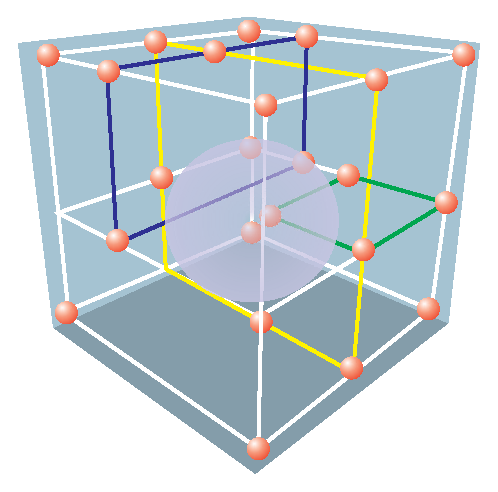
\includegraphics[width=0.3\textwidth]{./04-figuras/figkdtree}
    \fonte{\citeonline{CELSO2012}}
    \label{fig:kdtree}
\end{figure}

\section{Quadros e Tabelas}
\label{sec:tabelas}

Também é apresentado o exemplo do \autoref{qua:comparabd} e da \autoref{tab:correlacao}, que aparece automaticamente na lista de quadros e tabelas.
Informações sobre a construção de tabelas no LATEX podem ser encontradas na literatura especializada \cite{Lamport1986,Buerger1989,Kopka2003,Mittelbach2004}.

\begin{quadro}[!htb]
    \centering
    \caption{Hierarquia de restrições das questões.\label{qua:comparabd}}
    \begin{tabular}{|p{7cm}|p{7cm}|}
        \hline
        \textbf{BD Relacionais} & \textbf{BD Orientados a Objetos} \\
        \hline
        Os dados são passivos, ou seja, certas operações limitadas podem ser automaticamente acionadas quando os dados são usados. Os dados são ativos, ou seja, as solicitações fazem com que os objetos executem seus métodos. & Os processos que usam dados mudam constantemente. \\
        \hline
    \end{tabular}
    \fonte{\citeonline{carvalho:2001}}
\end{quadro}


Muitos confundem, mas existe diferença entre tabelas e quadros.
Um quadro é formado por linhas horizontais e verticais,
sendo, portanto ``fechado''. Normalmente é usado
para apresentar dados secundários. Nada impede, porém,
que um quadro apresente resultados da pesquisa.
Um quadro normalmente apresenta resultados
qualitativos (textos). O número do quadro e o título
vêm acima do quadro, e a fonte, deve vir abaixo.
Uma tabela é formada apenas por linhas verticais, sendo,
portanto ``aberta''. Normalmente é usada para
apresentar dados primários, e geralmente vem nos
“resultados” e na discussão do trabalho. Nada
impede, porém, que uma tabela seja usada no
referencial teórico de um trabalho. Uma tabela
normalmente apresenta resultados quantitativos
(números). O número da tabela e o título vêm
acima da tabela, e a fonte, deve vir abaixo, como
no quadro.

Exemplos de tabelas:

\begin{table}[!htb]
	\centering
	\begin{tabular}{cc}
		\hline
			x & y \\
		\hline
			1 & 2 \\
			3 & 4 \\
			5 & 6 \\
			7 & 8 \\
		\hline
	\end{tabular}
	\caption[Correlação de valores x e y]{Exemplo de uma tabela mostrando a correlação entre x e y.\label{tab:correlacao}}
%	\fonte{Autoria própria.}
\end{table}


\begin{table}[!htb]
    \centering
    \caption[Resultado dos testes]{Resultado dos testes.\label{tab:testes}}
    \begin{tabular}{rrrrr}
        \toprule
            & Valores 1 & Valores 2 & Valores 3 & Valores 4 \\
        \midrule
            Caso 1 & 0,86 & 0,77 & 0,81 & 163 \\
            Caso 2 & 0,19 & 0,74 & 0,25 & 180 \\
            Caso 3 & 1,00 & 1,00 & 1,00 & 170 \\
        \bottomrule
    \end{tabular}
\end{table}


\section{Equações}
\label{sec:equacoes}

A transformada de Laplace é dada na \autoref{eq:laplace}, enquanto a \autoref{eq:dft} apresenta a formulação da transformada discreta de Fourier bidimensional\footnote{Deve-se reparar na formatação esteticamente perfeita destas equações.}.

\begin{equation}
    X(s) = \int\limits_{t = -\infty}^{\infty} x(t) \, \text{e}^{-st} \, dt
    \label{eq:laplace}
\end{equation}

\begin{equation}
    F(u, v) = \sum_{m = 0}^{M - 1} \sum_{n = 0}^{N - 1} f(m, n) \exp \left[ -j 2 \pi \left( \frac{u m}{M} + \frac{v n}{N} \right) \right]
    \label{eq:dft}
\end{equation}

\section{Algoritmos}\label{sec:algoritmos}

Os algoritmos devem ser feitos segundo o modelo abaixo.
Para isso, utilizar o pacote {\ttfamily algorithm2e} no início do arquivo principal como neste exemplo.
O \autoref{alg:vertices} mostra um exemplo.

\begin{algorithm}
\caption{Algoritmo para remoção aleatória de vértices}
\KwIn{o número $n$ de vértices a remover, grafo original $G(V, E)$}
\KwOut{grafo reduzido $G'(V,E)$}
$removidos \leftarrow 0$ \\
\While {removidos $<$ n } {
	$v \leftarrow$ Random$(1, ..., k) \in V$ \\
		\For {$u \in adjacentes(v)$} {
			remove aresta (u, v)\\
			$removidos \leftarrow removidos + 1$\\
		}
		\If {há  componentes desconectados} {
			remove os componentes desconectados\\
		}
	}
\end{algorithm}

	% Fundamentação teórica
	%
% Documento: Metodologia
%

\chapter{Metodologia}

Inserir seu texto aqui...

\section{Delineamento da pesquisa}

Inserir seu texto aqui...

\section{Coleta de dados}

Inserir seu texto aqui...

		% Metodologia
	%
% Documento: Resultados
%

\chapter{Análise de Resultados}

Inserir seu texto aqui...

\section{Situação atual}

Inserir seu texto aqui...

\section{Análise dos dados coletados}

Inserir seu texto aqui...

		% Resultados
	%
% Documento: Conclusão
%

\chapter{Conclusão}
\label{chap:conclusao}

Espera-se que o uso do estilo de formatação LATEX adequado às Normas para Elaboração de Trabalhos Acadêmicos do CEFET-MG ({\ttfamily abnt-cefetmg.cls}) facilite a escrita de documentos no âmbito desta instituição e aumente a produtividade de seus autores. Para usuários iniciantes em LATEX, além da bibliografia especializada já citada, existe ainda uma série de recursos \cite{CTAN2009} e fontes de informação \cite{TeX-Br2009,Wikibooks2009} disponíveis na Internet.

Recomenda-se o editor de textos Kile como ferramenta de composição de documentos em LATEX para usuários Linux. Para usuários Windows recomenda-se o editor TEXnicCenter \cite{TeXnicCenter2009}. O LATEX normalmente já faz parte da maioria das distribuições Linux, mas no sistema operacional Windows é necessário instalar o software MiKTeX \cite{MiKTeX2009}.

Além disso, recomenda-se o uso de um gerenciador de referências como o JabRef \cite{JabRef2009} ou Mendeley \cite{Mendeley2009} para a catalogação bibliográfica em um arquivo BIBTEX, de forma a facilitar citações através do comando \verb#\cite{}# e outros comandos correlatos do pacote ABNTEX. A lista de referências deste documento foi gerada automaticamente pelo software LATEX + BIBTEX a partir do arquivo {\ttfamily refbase.bib}, que por sua vez foi composto com o gerenciador de referências JabRef.

O estilo de formatação LATEX do CEFET-MG e este exemplo de utilização foi elaborado por
\href{mailto:cfgnunes@gmail.com}{Cristiano Fraga Guimarães Nunes},
baseado nos modelos criados por
\href{mdiogo.kuiaski@gmail.com}{Diogo Rosa Kuiaski} e \href{hvieir@utfpr.edu.br}{Hugo Vieira Neto}. Sugestões de melhoria são bem vindas.

\section{Trabalhos Futuros}
\label{sec:trabalhosFuturos}

Inserir seu texto aqui...
		% Conclusão

% elementos pós textuais
	\postextual
	%
% Documento: Referências Bibliográficas
%

\bibliography{./refbase}	% geracao automatica das referencias a partir do arquivo refbase.bib
	% Referências
	%\include{./03-elementos-pos-textuais/glossario}	% Glossário
	%
% Documento: Apêndice
%

\begin{apendicesenv}
\partapendices

\chapter{Nome do Apêndice}
\label{chap:apendicex}

Inserir seu texto aqui...

\chapter{Nome do Apêndice}
\label{chap:apendicey}

Inserir seu texto aqui...

\end{apendicesenv}		% Apêndices
	%
% Documento: Anexos
%

\begin{anexosenv}
\partanexos

\chapter{Nome do anexo}
\label{chap:anexox}

Inserir seu texto aqui...

\chapter{Nome do anexo}
\label{chap:anexoy}

Inserir seu texto aqui...

\end{anexosenv}		% Anexos
	%\include{./03-elementos-pos-textuais/indices}		% Índices

\end{document}
